
%%% main document {{{

\documentclass[
a4paper,     %% defines the paper size: a4paper (default), a5paper, letterpaper, ...
% landscape,   %% sets the orientation to landscape
% twoside,     %% changes to a two-page-layout (alternatively: oneside)
% twocolumn,   %% changes to a two-column-layout
 headsepline, %% add a horizontal line below the column title
% footsepline, %% add a horizontal line above the page footer
% titlepage,   %% only the titlepage (using titlepage-environment) appears on the first page (alternatively: notitlepage)
% parskip,     %% insert an empty line between two paragraphs (alternatively: halfparskip, ...)
% leqno,       %% equation numbers left (instead of right)
% fleqn,       %% equation left-justified (instead of centered)
% tablecaptionabove, %% captions of tables are above the tables (alternatively: tablecaptionbelow)
% draft,       %% produce only a draft version (mark lines that need manual edition and don't show graphics)
% 10pt         %% set default font size to 10 point
11pt         %% set default font size to 11 point
% 12pt         %% set default font size to 12 point
]{scrartcl}  %% article, see KOMA documentation (scrguide.dvi)



%%%%%%%%%%%%%%%%%%%%%%%%%%%%%%%%%%%%%%%%%%%%%%%%%%%%%%%%%%%%%%%%%%%%%%%%%%%%%%%%
%%%
%%% packages
%%%

%%%
%%% encoding and language set
%%%

%%% ngerman: language set to new-german
\usepackage{ngerman}

%%% babel: language set (can cause some conflicts with package ngerman)
%%%        use it only for multi-language documents or non-german ones
%\usepackage[ngerman]{babel}

%%% inputenc: coding of german special characters
\usepackage[utf8]{inputenc}

%%% fontenc, ae, aecompl: coding of characters in PDF documents
\usepackage[T1]{fontenc}
\usepackage{ae,aecompl}

%%%
%%% technical packages
%%%

%%% amsmath, amssymb, amstext: support for mathematics
%\usepackage{amsmath,amssymb,amstext}

%%% psfrag: replace PostScript fonts
\usepackage{psfrag}

%%% listings: include programming code
%\usepackage{listings}

%%% units: technical units
\usepackage{units}

%%% tiefgestellte zahlen
\usepackage{subscript}

%%% mathefoo
\usepackage{amsmath}

%%% landscape page
\usepackage{pdflscape}

\usepackage{xcolor}
% TikZ-Bibliotheken
\usepackage{tikz}
 \usetikzlibrary{backgrounds}
 \usetikzlibrary{matrix}
 \usetikzlibrary{circuits.ee.IEC}
 \usetikzlibrary{positioning}
 
 
%Hintergrundstyle - optional
\tikzstyle{background rectangle}=
  [thick,draw=\lightgray, fill=white!99!black, rounded corners]
 
%Volt- und Amperemeter festlegen:
\tikzset{circuit declare symbol = ammeter}
\tikzset{set ammeter graphic ={draw,generic circle IEC, minimum size=5mm,info=center:A}}
\tikzset{circuit declare symbol = voltmeter}
\tikzset{set voltmeter graphic ={draw,generic circle IEC, minimum size=5mm,info=center:V}}
\tikzset{circuit declare symbol = generator}
\tikzset{set generator graphic ={draw,rectangle ee, minimum size=5mm,info=center:G}}
% Spannungs und Strompfeile
\tikzset{
  Pfeil/.style={thick,shorten >=#1,shorten <=#1,->}, % für Peile
  UPfeil/.style={blue,Pfeil=#1,font={\sffamily\itshape}},% für Spannungspfeile
  IPfeil/.style={red,Pfeil=#1,font={\ttfamily\itshape}} % für Strompfeile
}


%Boxen
\usepackage{empheq}
 
% Command "alignedbox{}{}" for a box within an align environment
% Source: http://www.latex-community.org/forum/viewtopic.php?f=46&t=8144
\newlength\dlf  % Define a new measure, dlf
\newcommand\alignedbox[2]{
% Argument #1 = before & if there were no box (lhs)
% Argument #2 = after & if there were no box (rhs)
&  % Alignment sign of the line
{
\settowidth\dlf{$\displaystyle #1$}  
    % The width of \dlf is the width of the lhs, with a displaystyle font
\addtolength\dlf{\fboxsep+\fboxrule}  
    % Add to it the distance to the box, and the width of the line of the box
\hspace{-\dlf}  
    % Move everything dlf units to the left, so that & #1 #2 is aligned under #1 & #2
\boxed{#1 #2}
    % Put a box around lhs and rhs
}
}

%%%
%%% layout
%%%

%%% scrpage2: KOMA heading and footer
%%% Note: if you don't use this package, please remove 
%%%       \pagestyle{scrheadings} and corresponding settings
%%%       below too.
\usepackage[automark]{scrpage2}


%%%
%%% PDF
%%%

\usepackage{ifpdf}

%%% Should be LAST usepackage-call!
%%% For docu on that, see reference on package ``hyperref''
\ifpdf%   (definitions for using pdflatex instead of latex)

  %%% graphicx: support for graphics
  %\usepackage[pdftex]{graphicx}

  \pdfcompresslevel=9

  %%% hyperref (hyperlinks in PDF): for more options or more detailed
  %%%          explanations, see the documentation of the hyperref-package
  \usepackage[%
    %%% general options
    pdftex=true,      %% sets up hyperref for use with the pdftex program
    %plainpages=false, %% set it to false, if pdflatex complains: ``destination with same identifier already exists''
    %
    %%% extension options
    backref,      %% adds a backlink text to the end of each item in the bibliography
    pagebackref=false, %% if true, creates backward references as a list of page numbers in the bibliography
    colorlinks=true,   %% turn on colored links (true is better for on-screen reading, false is better for printout versions)
    %
    %%% PDF-specific display options
    bookmarks=true,          %% if true, generate PDF bookmarks (requires two passes of pdflatex)
    bookmarksopen=false,     %% if true, show all PDF bookmarks expanded
    bookmarksnumbered=false, %% if true, add the section numbers to the bookmarks
    %pdfstartpage={1},        %% determines, on which page the PDF file is opened
    pdfpagemode=None         %% None, UseOutlines (=show bookmarks), UseThumbs (show thumbnails), FullScreen
  ]{hyperref}


  %%% provide all graphics (also) in this format, so you don't have
  %%% to add the file extensions to the \includegraphics-command
  %%% and/or you don't have to distinguish between generating
  %%% dvi/ps (through latex) and pdf (through pdflatex)
  \DeclareGraphicsExtensions{.pdf}

\else %else   (definitions for using latex instead of pdflatex)

  \usepackage[dvips]{graphicx}

  \DeclareGraphicsExtensions{.eps}

  \usepackage[%
    dvips,           %% sets up hyperref for use with the dvips driver
    colorlinks=false %% better for printout version; almost every hyperref-extension is eliminated by using dvips
  ]{hyperref}

\fi


%%% sets the PDF-Information options
%%% (see fields in Acrobat Reader: ``File -> Document properties -> Summary'')
%%% Note: this method is better than as options of the hyperref-package (options are expanded correctly)
\hypersetup{
  pdftitle={}, %%
  pdfauthor={}, %%
  pdfsubject={}, %%
  pdfcreator={Accomplished with LaTeX2e and pdfLaTeX with hyperref-package.}, %% 
  pdfproducer={}, %%
  pdfkeywords={} %%
}


%%%%%%%%%%%%%%%%%%%%%%%%%%%%%%%%%%%%%%%%%%%%%%%%%%%%%%%%%%%%%%%%%%%%%%%%%%%%%%%%
%%%
%%% user defined commands
%%%

%%% \mygraphics{}{}{}
%% usage:   \mygraphics{width}{filename_without_extension}{caption}
%% example: \mygraphics{0.7\textwidth}{rolling_grandma}{This is my grandmother on inlinescates}
%% requires: package graphicx
%% provides: including centered pictures/graphics with a boldfaced caption below
%% 
\newcommand{\mygraphics}[3]{
  \begin{center}
    \includegraphics[width=#1, keepaspectratio=true]{#2} \\
    \textbf{#3}
  \end{center}
}

%%%%%%%%%%%%%%%%%%%%%%%%%%%%%%%%%%%%%%%%%%%%%%%%%%%%%%%%%%%%%%%%%%%%%%%%%%%%%%%%
%%%
%%% define the titlepage
%%%

% \subject{}   %% subject which appears above titlehead
% \titlehead{} %% special heading for the titlepage

%%% title
\title{Messbericht \\ Kondensator an Gleichspannung}

%%% author(s)
\author{Felix Schiller \\ Sebastian Littau \\ E1FS2}

%%% date
\date{Reutlingen, am 08.03.2015}

% \publishers{}

% \thanks{} %% use it instead of footnotes (only on titlepage)

% \dedication{} %% generates a dedication-page after titlepage


%%% uncomment following lines, if you want to:
%%% reuse the maketitle-entries for hyperref-setup
%\newcommand\org@maketitle{}
%\let\org@maketitle\maketitle
%\def\maketitle{%
%  \hypersetup{
%    pdftitle={\@title},
%    pdfauthor={\@author}
%    pdfsubject={\@subject}
%  }%
%  \org@maketitle
%}


%%%%%%%%%%%%%%%%%%%%%%%%%%%%%%%%%%%%%%%%%%%%%%%%%%%%%%%%%%%%%%%%%%%%%%%%%%%%%%%%
%%%
%%% set heading and footer
%%%

%%% scrheadings default: 
%%%      footer - middle: page number
\pagestyle{scrheadings}

%%% user specific
%%% usage:
%%% \position[heading/footer for the titlepage]{heading/footer for the rest of the document}

%%% heading - left
\ihead[]{Schiller, Felix \\ Littau, Sebastian}

%%% heading - center
\chead[]{Messbericht \\ Kondensator an Gleichspannung}

%%% heading - right
\ohead[]{\thepage}

%%% footer - left
% \ifoot[]{}

%%% footer - center
% \cfoot[]{}

%%% footer - right
% \ofoot[]{}



%%%%%%%%%%%%%%%%%%%%%%%%%%%%%%%%%%%%%%%%%%%%%%%%%%%%%%%%%%%%%%%%%%%%%%%%%%%%%%%%
%%%
%%% begin document
%%%

\begin{document}

% \pagenumbering{roman} %% small roman page numbers

%%% include the title
% \thispagestyle{empty}  %% no header/footer (only) on this page
\maketitle

%%% start a new page and display the table of contents
\newpage
\tableofcontents

%%% start a new page and display the list of figures
% \newpage
% \listoffigures

%%% start a new page and display the list of tables
% \newpage
% \listoftables

%%% display the main document on a new page 
% \newpage

% \pagenumbering{arabic} %% normal page numbers (include it, if roman was used above)

%%%%%%%%%%%%%%%%%%%%%%%%%%%%%%%%%%%%%%%%%%%%%%%%%%%%%%%%%%%%%%%%%%%%%%%%%%%%%%%%
%%%
%%% begin main document
%%% structure: \section \subsection \subsubsection \paragraph \subparagraph
%%%
\section{Messaufgabe}
Ein Kondensator wirkt in einem Gleichstromkreis wie eine Unterbrechung und als Ladungsspeicher. Sowohl beim Laden als auch beim Entladen des Kondensators fließt ein Strom nur für eine bestimmte Zeit.

\section{Durchführung der Messung}
\subsection{Spannungsmessung am Kondensator}
Die wichtigsten ungepolten Kondensatorarten sind Keramikkondensatoren, Kunststoff-Folienkondensatoren, und Wickelkondensatoren. Die wichtigsten Vertreter der gepolten Variante sind die Tantal- und Elektrolytkondensatoren. Obwohl sie auf völlig anderen Speicherprinzipien beruhen gehören die Superkondensatoren ebenfalls dazu. Neben diesen Kondensatoren mit festen Kapazitätswerten gibt es Bauelemente mit einstellbaren Kapazitätswerten, die variablen Kondensatoren.
Typische Kondensatoren haben Kapazitäten im Bereich von wenigen piko-Farad bis hin zu mehreren milli-Farad.
\begin{center}
\begin{tabular}{ c | c | c }
    \hline
    mF  & milli Farad & $10^{-3}$ \\ \hline
    $\mu$F  & mikro Farad & $10^{-6}$ \\ \hline
    nF  & nano Farad  & $10^{-9}$ \\ \hline
    pF  & piko Farad  & $10^{-12}$ \\
    \hline
\end{tabular}
\end{center}
Die Schaltzeichen für Kondensatoren sind genormt. Je nach Typ werden verschiedene Schaltzeichen verwendet.
\begin{figure}
\centering
\def\svgwidth{\columnwidth}
\input{Kondensatoren-Schaltzeichen-Reihe.pdf_tex}
\end{figure}



\subsection{Messschaltung}
\begin{center}
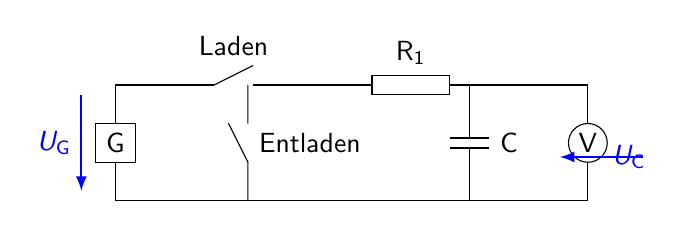
\begin{tikzpicture}[%show background rectangle,
circuit ee IEC, circuit symbol lines/.style={draw,thick},
font=\sffamily\upshape,
>=latex % Voreinstellung für Pfeilspitzen
]
\matrix (S) [
  matrix of nodes, nodes in empty cells,
  inner sep=0pt, outer sep=-.5\pgflinewidth,
  column sep=15mm, row sep = 7mm,
  nodes={minimum width=0pt}
  ]
{
  &&&&  \\
  &&&&  \\
  &&&&  \\
};
 
 
%Orientierungshilfen
%\foreach \j in {1,...,3}
%{
%	\foreach \k in {1,...,5}
%	{%
%		\node[text=lightgray] at (S-\j-\k){+}; % Orientierungshilfe +
%		\node[red, left] at (S-\j-1){\j}; %Orientierungshilfe Zeilennummer
%		\node[red, above] at (S-1-\k){\k}; %Orientierungshilfe Spaltennummer  
%	};%
%}

%Bauteile
\draw (S-3-1) to  [generator={name=Gen}](S-1-1);

\draw (S-1-1) to  [make contact={info=Laden, name=switch}](S-1-3);
\draw ([xshift=.52em]S-3-2.center) to  [make contact={info'=Entladen, name=switch}]([xshift=.52em]S-1-2.center);
\draw (S-1-3) to  [resistor={info=R$_\mathsf{1}$, name=Wstd1}](S-1-4);
\draw (S-1-4) to  [capacitor={info=C}](S-3-4);
\draw (S-1-5) to  [voltmeter={name=VM1}](S-3-5);

%Spannungspfeile
%Spannungspfeil der Quelle / des Voltmeters
\draw[UPfeil=-1em]([xshift=-.5em]Gen.north west) -- node [left]{U$\mathsf{_G}$}([xshift=-.5em]Gen.south west);
\draw[UPfeil=-1em]([xshift=.5em]VM1.north east) -- node [right]{U$\mathsf{_C}$}([xshift=.5em]VM1.south east);


%Strompfeile
%\draw[IPfeil=-1em]([yshift=.5em]AM1.north west) -- node [above]{I$\mathsf{_L}$}([yshift=.5em]AM1.north east);

 
%Leiterbahnen

%\draw (S-1-1) -- (S-1-2);
\draw (S-1-4) -- (S-1-5);
\draw (S-3-1) -- (S-3-5);

%\draw [dashed]([xshift=-2.8em, yshift=2em]S-1-1.center) -- ([yshift=2em]S-1-2.center);
%\draw [dashed]([xshift=-2.8em, yshift=2em]S-1-1.center) -- ([xshift=-2.8em, yshift=-2em]S-3-1.center);
%\draw [dashed]([yshift=2em]S-1-2.center) -- ([yshift=-2em]S-3-2.center); 
%\draw [dashed]([xshift=-2.8em, yshift=-2em]S-3-1.center) -- ([yshift=-2em]S-3-2.center); 
 
\end{tikzpicture}
\end{center}

\subsection{Aufbau der Schaltung}
In der obigen Messschaltung wird ein Kondensator mit einer Kapazität von $C=60\mu F$ über einen Vorwiderstand von $R1=220k\Omega$ auf- und entladen. Die Umschaltung von Laden auf Entladen erfolgt über die beiden Schalter. In zwei Messdurchgängen wird die Generatorspannung auf $U_G=8V$ bzw. $U_G=16V$ eingestellt. Die Spannung $U_C$ am Kondensator wird mit einem präzisen und schnellen Tischmultimeter gemessen.

\subsection{Laden und entladen des Kondensators}

In einem ersten Messdurchgang wird der Kondensator geladen. Der momentane Spannungswert $U_C$ am Kondensator wird in 5s Abständen bis 30s und in 10s Abständen bis 90s notiert. Nach den ersten 90s werden die Schalter auf Entladung umgelegt und die Messwerte wieder zu den gleichen Zeitpunkten notiert. 

\subsection{Messwerttabelle}
\begin{center}
\begin{tabular}{ r | r | r | r | r }
	\multicolumn{1}{r}{} &  \multicolumn{2}{|c}{$U_C$ bei $8V$} & \multicolumn{2}{|c}{$U_C$ bei $16V$} \\ \hline
    $t$ in s    & Laden & Entladen & Laden & Entladen \\ \hline
    0           & 0     & 7.5      & 0     & 15.54 \\
    5           & 2.5   & 5.1      & 4.7   & 11.1 \\
    10          & 4.2   & 3.5      & 8.1   & 7.4 \\
    15          & 5.4   & 2.4      & 10.6  & 5.3 \\
    20          & 6.25  & 1.7      & 12.1  & 3.5 \\
    25          & 6.7   & 1.18     & 13.1  & 2.5 \\
    30          & 7.02  & 0.8      & 13.9  & 1.74 \\
    40          & 7.45  & 0.4      & 14.83 & 0.83 \\
    50          & 7.64  & 0.18     & 15.26 & 0.39 \\
    60          & 7.75  & 0.089    & 15.46 & 0.184 \\
    70          & 7.79  & 0.042    & 15.56 & 0.089 \\
    80          & 7.81  & 0.020    & 15.61 & 0.043 \\
    90          & 7.82  & 0.009    & 15.63 & 0.02 \\
    \hline
\end{tabular} \\
\end{center}

\begin{landscape}

\section{Grafische Auswertung}

\subsection{Theoretische und gemessene Kennlinie}
\begin{figure}[hbtp]
\centering
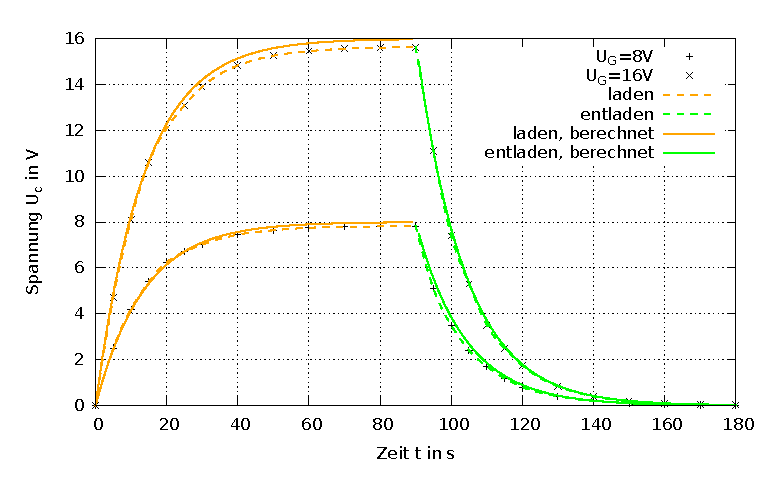
\includegraphics[scale=1.48]{kennlinie.eps}
\end{figure}

\end{landscape}

\subsection{Kurvenauswertung}
Die Lade- und Entladekurven folgen einer $e$-Funktion. Die eingestellte Generatorspannung von 8V bzw. 16V wird nie erreicht. Je näher sich die Kondensatorspannung $U_C$ und $U_G$ annähert, desto kleiner wird die Steigung der Kurve. Um die Zeit, die es braucht bis ein Kondensator als geladen gilt zu beschreiben wurde der Begriff $\tau$ eingeführt.
\begin{align}
\tau &=R \cdot C \nonumber \\
     &=\Omega \cdot F \nonumber \\
     &=\frac{V}{A} \cdot \frac{AS}{V} \nonumber \\
     &= s \nonumber
\end{align}
Nach $\tau$ Sekunden ist ein Kondensator zu 63\% aufgeladen. Nach $5\tau$ Sekunden gilt der Kondensator als vollständig geladen.\newline
Den genauen Ladezustand eines Kondensators bei idealen Bedingungen nach einer bestimmten Zeit lässt sich mit der folgenden Formel ausrechnen:
\[U_C = U_0 \cdot [1-e^{(-\frac{t}{\tau})}]\]
mit $\tau = R\cdot C = 224k\Omega \cdot 61.1\mu F=13.68s$
\[U_C = 8V \cdot [1-e^{(-\frac{t}{13.68s})}]\]
Für das Entladen gilt:
\[U_C = U_0 \cdot [e^{(-\frac{t}{\tau})}]\]
Über diese Funktionen sind die berechneten Kennlinien im obigen Diagramm erstellt worden.

%%%
%%% end main document
%%%
%%%%%%%%%%%%%%%%%%%%%%%%%%%%%%%%%%%%%%%%%%%%%%%%%%%%%%%%%%%%%%%%%%%%%%%%%%%%%%%%

% \appendix  %% include it, if something (bibliography, index, ...) follows below

%%%%%%%%%%%%%%%%%%%%%%%%%%%%%%%%%%%%%%%%%%%%%%%%%%%%%%%%%%%%%%%%%%%%%%%%%%%%%%%%
%%%
%%% bibliography
%%%
%%% available styles: abbrv, acm, alpha, apalike, ieeetr, plain, siam, unsrt
%%%
% \bibliographystyle{plain}

%%% name of the bibliography file without .bib
%%% e.g.: literatur.bib -> \bibliography{literatur}
% \bibliography{FIXXME}

\end{document}
%%% }}}
%%% END OF FILE
%%%%%%%%%%%%%%%%%%%%%%%%%%%%%%%%%%%%%%%%%%%%%%%%%%%%%%%%%%%%%%%%%%%%%%%%%%%%%%%%
%%% Notice!
%%% This file uses the outline-mode of emacs and the foldmethod of Vim.
%%% Press 'zi' to unfold the file in Vim.
%%% See ':help folding' for more information.
%%%%%%%%%%%%%%%%%%%%%%%%%%%%%%%%%%%%%%%%%%%%%%%%%%%%%%%%%%%%%%%%%%%%%%%%%%%%%%%%
%% Local Variables:
%% mode: outline-minor
%% OPToutline-regexp: "%% .*"
%% OPTeval: (hide-body)
%% emerge-set-combine-versions-template: "%a\n%b\n"
%% End:
%% vim:foldmethod=marker
